%%%%%%%%%%%%%%%%%%%%%%%%%%%%%%%%%%%%%%%%%%%%%%%%%%%%%%%%%%%%%%%%%%%%%%%%%%%%%%%%%%%%%%%%
% Setup I6pd2 style, common packages
%%%%%%%%%%%%%%%%%%%%%%%%%%%%%%%%%%%%%%%%%%%%%%%%%%%%%%%%%%%%%%%%%%%%%%%%%%%%%%%%%%%%%%%%
\documentclass[final,hyperref={pdfpagelabels=false},noamsthm]{beamer}
\usepackage{default}

\usetheme{I6pd2} % Use the I6pd2 theme supplied with this template

\usepackage[english]{babel} % English language/hyphenation

\usepackage{amsmath,amsthm}

\usepackage{tikz}
\usetikzlibrary{fit}					% fitting shapes to coordinates
\usetikzlibrary{backgrounds}	% drawing the background after the foreground

%%%%%%%%%%%%%%%%%%%%%%%%%%%%%%%%%%%%%%%%%%%%%%%%%%%%%%%%%%%%%%%%%%%%%%%%%%%%%%%%%%%%%%%%
% Shortcuts for this project
%%%%%%%%%%%%%%%%%%%%%%%%%%%%%%%%%%%%%%%%%%%%%%%%%%%%%%%%%%%%%%%%%%%%%%%%%%%%%%%%%%%%%%%%

% blackboard series
\def\bbP{\mathbb{P}}
\def\bbp{\mathbb{p}}
\def\bbE{\mathbb{E}}
\def\bbN{\mathbb{N}}

% calligraphic series
\def\calT{\mathcal{T}}
\def\calW{\mathcal{W}}
\def\calX{\mathcal{X}}

% bold series
\def\bfP{\mathbf{P}}
\def\bfX{\mathbf{X}}

% distributions
\def\aDist{\Lambda}
\def\aTime{T}
\def\Geom{\text{Geom}}

% stuff
\newcommand{\prob}{\mathbb{P}}
\newcommand{\calV}{\mathcal{V}}
\newcommand{\calE}{\mathcal{E}}
\newcommand{\ee}{Z} % ends of edges
\newcommand{\bfee}{\mathbf{\ee}}
\newcommand{\bfE}{\mathbf{E}}
\newcommand{\PYP}{\mathcal{PYP}}
\newcommand{\geom}{\beta}
\newcommand{\BNTL}{\text{\rm BNTL}}
\newcommand{\bfT}{\mathbf{T}}
\newcommand{\calO}{\mathcal{O}}
\newcommand{\bbR}{\mathbb{R}}
\newcommand{\bfPsi}{\boldsymbol{\Psi}}
\newcommand{\bfn}{\mathbf{n}}
\newcommand{\bfd}{\mathbf{d}}
\newcommand{\argdot}{{\,\vcenter{\hbox{\scalebox{0.5}{$\bullet$}}}\,}}%{\bullet}
\def\indicator{\mathbf{1}}
\newcommand{\limscale}[2]{\overset{\scriptscriptstyle{#1 \uparrow #2}}{\widesim[1.25]}}
\newcommand{\simiid}{\overset{\scriptscriptstyle{\text{i.i.d.}}}{\widesim}}
\newcommand{\widesim}[1][1.5]{
	\mathrel{\scalebox{#1}[1]{$\sim$}}
}

%%%%%%%%%%%%%%%%%%%%%%%%%%%%%%%%%%%%%%%%%%%%%%%%%%%%%%%%%%%%%%%%%%%%%%%%%%%%%%%%%%%%%%%%
% Define footer contents
%%%%%%%%%%%%%%%%%%%%%%%%%%%%%%%%%%%%%%%%%%%%%%%%%%%%%%%%%%%%%%%%%%%%%%%%%%%%%%%%%%%%%%%%

\newcommand{\leftfoot}{} % Left footer text

\newcommand{\rightfoot}{~ \url{http://csml.stats.ox.ac.uk/learning/}} % Right footer text


\title{Sampling and Inference for Beta Neutral-to-the-Left Models of Sparse Networks} % Poster title

\author{Benjamin Bloem-Reddy, \underline{Adam Foster}, Emile Mathieu, Yee Whye Teh }
\institute{Department of Statistics, University of Oxford}

%%%%%%%%%%%%%%%%%%%%%%%%%%%%%%%%%%%%%%%%%%%%%%%%%%%%%%%%%%%%%%%%%%%%%%%%%%%%%%%%%%%%%%%%
% Main presentation
%%%%%%%%%%%%%%%%%%%%%%%%%%%%%%%%%%%%%%%%%%%%%%%%%%%%%%%%%%%%%%%%%%%%%%%%%%%%%%%%%%%%%%%%

\begin{document}
	
\begin{frame}[plain]
	\titlepage
\end{frame}

\begin{frame}
	\frametitle{Contents}
	\tableofcontents
\end{frame}

\section{Background}
\subsection{Temporal networks}

\begin{frame}
	\frametitle{Temporal networks}
	\textbf{Examples}
	\begin{itemize}
		\item Messages on WhatsApp
		\item Posts + replies on StackOverflow
	\end{itemize}
	\vspace{15pt}
	\textbf{Abstraction}
	\begin{itemize}
		\item Graph grows adding one edge $(Z_i, Z_{i+1})$ at a time
		\item Vertices enter the graph when connected to
	\end{itemize}
	
\end{frame}

\begin{frame}
	\frametitle{Temporal networks}
	Ends of edges $\mathbf{Z}_n = Z_1, ..., Z_n$ \\
	E.g. $\mathbf{Z}_6 = \underline{a,b},\underline{c,a},\underline{d,e}$
	\begin{figure}[H]
		\begin{center}
			% ,>=stealth',shorten >=1pt,
			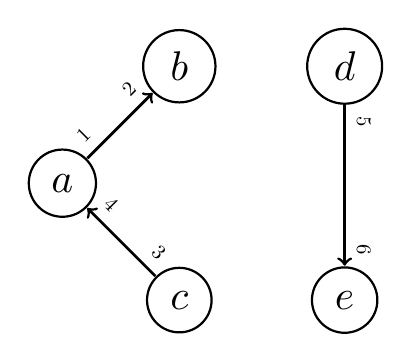
\begin{tikzpicture}[->,auto,node distance=1.4cm, thick,baseline=0]
			\tikzstyle{every node}=[shape=circle,draw=black,text=black,scale=1.5]
			\tikzstyle{every edge}=[line width=1pt,draw=black]
			
			\node         (1)                    {$a$};
			\node         (2) [above right of=1] {$b$};
			\node         (3) [below right of=1] {$c$};
			\node         (4) [right of=2]       {$d$};
			\node         (5) [right of=3]       {$e$};
			
			\draw (1) edge node [pos=0.15, sloped, above, draw=none, scale=0.5] {1} node [pos=0.85, sloped, above, draw=none, scale=0.5] {2} (2);
			\draw (3) edge node [pos=0.15, sloped, above, draw=none, scale=0.5] {3} node [pos=0.85, sloped, above, draw=none, scale=0.5] {4} (1);
			\draw (4) edge node [pos=0.1, sloped, above, draw=none, scale=0.5] {5} node [pos=0.9, sloped, above, draw=none, scale=0.5] {6} (5);
			\end{tikzpicture}
			
		\end{center}
		%\caption{ Example graph: ends of edges $\mathbf{Z}_{6} = 1,2,\;3,1,\;4,5$, vertex arrival times $\mathbf{T}_{5} = 1, 2, 3, 5, 6$, vertex counts $\mathbf{K}_{6} = 1, 2, \; 3, 3, \; 4, 5$, and degree counts $m_6(1) = 4, m_6(2) = 1$.}
	\end{figure}
\end{frame}

\begin{frame}
	\frametitle{Temporal networks}
	Number of vertices $K_n$ \\
	E.g. $K_6 = 5$
	\begin{figure}[H]
		\begin{center}
			% ,>=stealth',shorten >=1pt,
			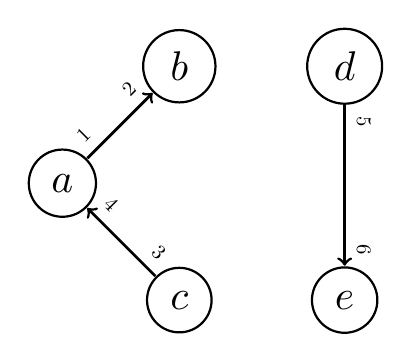
\begin{tikzpicture}[->,auto,node distance=1.4cm, thick,baseline=0]
			\tikzstyle{every node}=[shape=circle,draw=black,text=black,scale=1.5]
			\tikzstyle{every edge}=[line width=1pt,draw=black]
			
			\node         (1)                    {$a$};
			\node         (2) [above right of=1] {$b$};
			\node         (3) [below right of=1] {$c$};
			\node         (4) [right of=2]       {$d$};
			\node         (5) [right of=3]       {$e$};
			
			\draw (1) edge node [pos=0.15, sloped, above, draw=none, scale=0.5] {1} node [pos=0.85, sloped, above, draw=none, scale=0.5] {2} (2);
			\draw (3) edge node [pos=0.15, sloped, above, draw=none, scale=0.5] {3} node [pos=0.85, sloped, above, draw=none, scale=0.5] {4} (1);
			\draw (4) edge node [pos=0.1, sloped, above, draw=none, scale=0.5] {5} node [pos=0.9, sloped, above, draw=none, scale=0.5] {6} (5);
			\end{tikzpicture}
			
		\end{center}
		%\caption{ Example graph: ends of edges $\mathbf{Z}_{6} = 1,2,\;3,1,\;4,5$, vertex arrival times $\mathbf{T}_{5} = 1, 2, 3, 5, 6$, vertex counts $\mathbf{K}_{6} = 1, 2, \; 3, 3, \; 4, 5$, and degree counts $m_6(1) = 4, m_6(2) = 1$.}
	\end{figure}
\end{frame}

\begin{frame}
	\frametitle{Temporal networks}
	Arrival time of vertex $j$ is $T_j := \inf \{n: Z_n = j\}$ \\
	E.g. $T_e = 6$
	\begin{figure}[H]
		\begin{center}
			% ,>=stealth',shorten >=1pt,
			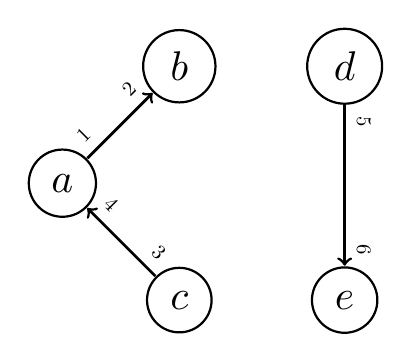
\begin{tikzpicture}[->,auto,node distance=1.4cm, thick,baseline=0]
			\tikzstyle{every node}=[shape=circle,draw=black,text=black,scale=1.5]
			\tikzstyle{every edge}=[line width=1pt,draw=black]
			
			\node         (1)                    {$a$};
			\node         (2) [above right of=1] {$b$};
			\node         (3) [below right of=1] {$c$};
			\node         (4) [right of=2]       {$d$};
			\node         (5) [right of=3]       {$e$};
			
			\draw (1) edge node [pos=0.15, sloped, above, draw=none, scale=0.5] {1} node [pos=0.85, sloped, above, draw=none, scale=0.5] {2} (2);
			\draw (3) edge node [pos=0.15, sloped, above, draw=none, scale=0.5] {3} node [pos=0.85, sloped, above, draw=none, scale=0.5] {4} (1);
			\draw (4) edge node [pos=0.1, sloped, above, draw=none, scale=0.5] {5} node [pos=0.9, sloped, above, draw=none, scale=0.5] {6} (5);
			\end{tikzpicture}
			
		\end{center}
		%\caption{ Example graph: ends of edges $\mathbf{Z}_{6} = 1,2,\;3,1,\;4,5$, vertex arrival times $\mathbf{T}_{5} = 1, 2, 3, 5, 6$, vertex counts $\mathbf{K}_{6} = 1, 2, \; 3, 3, \; 4, 5$, and degree counts $m_6(1) = 4, m_6(2) = 1$.}
	\end{figure}
\end{frame}

\begin{frame}
	\frametitle{Temporal networks}
	Degree of vertex $j$ is $d_{j,n}$ \\
	E.g. $d_{e,6} = 1$
	\begin{figure}[H]
		\begin{center}
			% ,>=stealth',shorten >=1pt,
			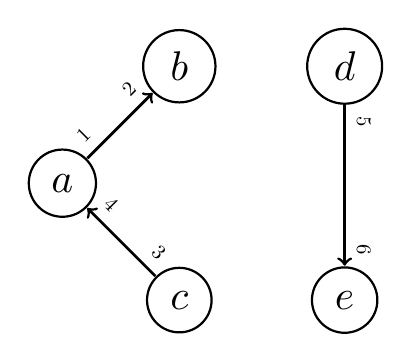
\begin{tikzpicture}[->,auto,node distance=1.4cm, thick,baseline=0]
			\tikzstyle{every node}=[shape=circle,draw=black,text=black,scale=1.5]
			\tikzstyle{every edge}=[line width=1pt,draw=black]
			
			\node         (1)                    {$a$};
			\node         (2) [above right of=1] {$b$};
			\node         (3) [below right of=1] {$c$};
			\node         (4) [right of=2]       {$d$};
			\node         (5) [right of=3]       {$e$};
			
			\draw (1) edge node [pos=0.15, sloped, above, draw=none, scale=0.5] {1} node [pos=0.85, sloped, above, draw=none, scale=0.5] {2} (2);
			\draw (3) edge node [pos=0.15, sloped, above, draw=none, scale=0.5] {3} node [pos=0.85, sloped, above, draw=none, scale=0.5] {4} (1);
			\draw (4) edge node [pos=0.1, sloped, above, draw=none, scale=0.5] {5} node [pos=0.9, sloped, above, draw=none, scale=0.5] {6} (5);
			\end{tikzpicture}
			
		\end{center}
		%\caption{ Example graph: ends of edges $\mathbf{Z}_{6} = 1,2,\;3,1,\;4,5$, vertex arrival times $\mathbf{T}_{5} = 1, 2, 3, 5, 6$, vertex counts $\mathbf{K}_{6} = 1, 2, \; 3, 3, \; 4, 5$, and degree counts $m_6(1) = 4, m_6(2) = 1$.}
	\end{figure}
\end{frame}

\begin{frame}
	\frametitle{Temporal networks}
	Degree counts $m_n(d) := |\{j: d_{j,n} = d\}|$ \\
	E.g. $m_6(1) = 4, m_6(2) = 1$
	\begin{figure}[H]
		\begin{center}
			% ,>=stealth',shorten >=1pt,
			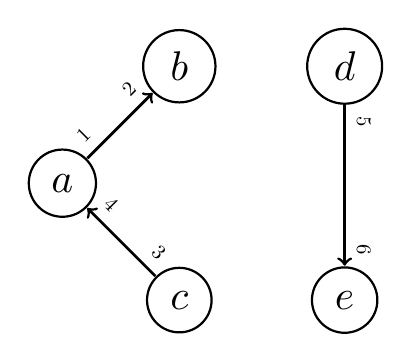
\begin{tikzpicture}[->,auto,node distance=1.4cm, thick,baseline=0]
			\tikzstyle{every node}=[shape=circle,draw=black,text=black,scale=1.5]
			\tikzstyle{every edge}=[line width=1pt,draw=black]
			
			\node         (1)                    {$a$};
			\node         (2) [above right of=1] {$b$};
			\node         (3) [below right of=1] {$c$};
			\node         (4) [right of=2]       {$d$};
			\node         (5) [right of=3]       {$e$};
			
			\draw (1) edge node [pos=0.15, sloped, above, draw=none, scale=0.5] {1} node [pos=0.85, sloped, above, draw=none, scale=0.5] {2} (2);
			\draw (3) edge node [pos=0.15, sloped, above, draw=none, scale=0.5] {3} node [pos=0.85, sloped, above, draw=none, scale=0.5] {4} (1);
			\draw (4) edge node [pos=0.1, sloped, above, draw=none, scale=0.5] {5} node [pos=0.9, sloped, above, draw=none, scale=0.5] {6} (5);
			\end{tikzpicture}
			
		\end{center}
		%\caption{ Example graph: ends of edges $\mathbf{Z}_{6} = 1,2,\;3,1,\;4,5$, vertex arrival times $\mathbf{T}_{5} = 1, 2, 3, 5, 6$, vertex counts $\mathbf{K}_{6} = 1, 2, \; 3, 3, \; 4, 5$, and degree counts $m_6(1) = 4, m_6(2) = 1$.}
	\end{figure}
\end{frame}



\subsection{Asymptotic properties}
\begin{frame}
	\frametitle{Sparsity}
	\begin{itemize}
		\item For a dense graph, $K_n = O(n^{1/2})$
		\item For a sparse graph,
		\begin{equation*}
			K_n = O(n^{1/(1+\sigma)})
		\end{equation*}
		for $0 \le \sigma < 1$
		\item Stack Overflow network likely sparse
	\end{itemize}
\end{frame}

\begin{frame}
	\frametitle{Power law degree distribution}
	A power law distribution of exponent $\eta$ on $\{1, 2, ...\}$ has
	\begin{equation*}
	p(d) \propto d^{-\eta} 
	\end{equation*}
	where $\eta > 1$.
	
	\pause
	The asymptotic degree distribution has \textbf{power law tail with exponent} $\eta > 1$ if
	\begin{align} 
	\label{eq:plaw}
	\frac{m_{n}(d)}{K_n} \xrightarrow[n\to\infty]{p} L(d)d^{-\eta} \;,
	\end{align}
	for slowly varying function $L(d)$.
\end{frame}

\begin{frame}
	\frametitle{Power laws and sparsity}
	We have
	\begin{align*}
		K_n &= \sum_{d=1}^\infty m_n(d), \\
		n &= \sum_{d=1}^\infty d\, m_n(d).
	\end{align*}
	Suppose (somewhat informally) that
	\begin{equation*}
		K_n = C_{n, \eta} \sum_{d=1}^n d^{-\eta}
	\end{equation*}
	\pause
	then 
	\begin{equation*}	
	n = C_{n, \eta} \sum_{d=1}^n d^{-\eta + 1} = K_n \, \frac{\sum_{d=1}^n d^{-\eta + 1}}{\sum_{d=1}^n d^{-\eta}}
	\end{equation*}
\end{frame}

\begin{frame}
	\frametitle{Power laws and sparsity}
	Letting $n\to \infty$ in
	\begin{equation*}
		\frac{K_n}{n} = \frac{\sum_{d=1}^n d^{-\eta}}{\sum_{d=1}^n d^{-\eta + 1}}
	\end{equation*}
	we see $K_n = O(n)$ if $\eta > 2$, $K_n = o(n)$ if $\eta \in (1, 2]$.
	\vspace{40pt}
	\pause
	
	\textbf{Summary}
	
	For sparse graphs, $\sigma=0 \leftrightarrow \eta > 2$ and $\sigma > 0 \leftrightarrow \eta \in (1,2]$.
\end{frame}

\subsection{Empirical study}
\begin{frame}
	\frametitle{Empirical study}
	\textbf{SNAP datasets} \cite{snapnets}
	\begin{table}[b]
		% \vspace*{-\baselineskip}
		\label{tab:datasets}
		\begin{center}
			\begin{tabular}{lll}
				Dataset                 & \# of vertices   & \# of edges    \\
				\hline
				Ask Ubuntu    & 159,316   & 964,437    \\
				UCI social network   & 1,899     & 20,296     \\
				EU email        & 986       & 332,334    \\
				Math Overflow & 24,818    & 506,550    \\
				Stack Overflow           & 2,601,977 & 63,497,050 \\
				Super User    & 194,085   & 1,443,339  \\
				Wikipedia talk pages    & 1,140,149 & 7,833,140 \\
			\end{tabular}
		\end{center}
	\end{table}
	
\end{frame}

\subsection{Empirical study}
\begin{frame}
	\frametitle{Ask Ubuntu arrival process}
	\begin{figure}[h]
		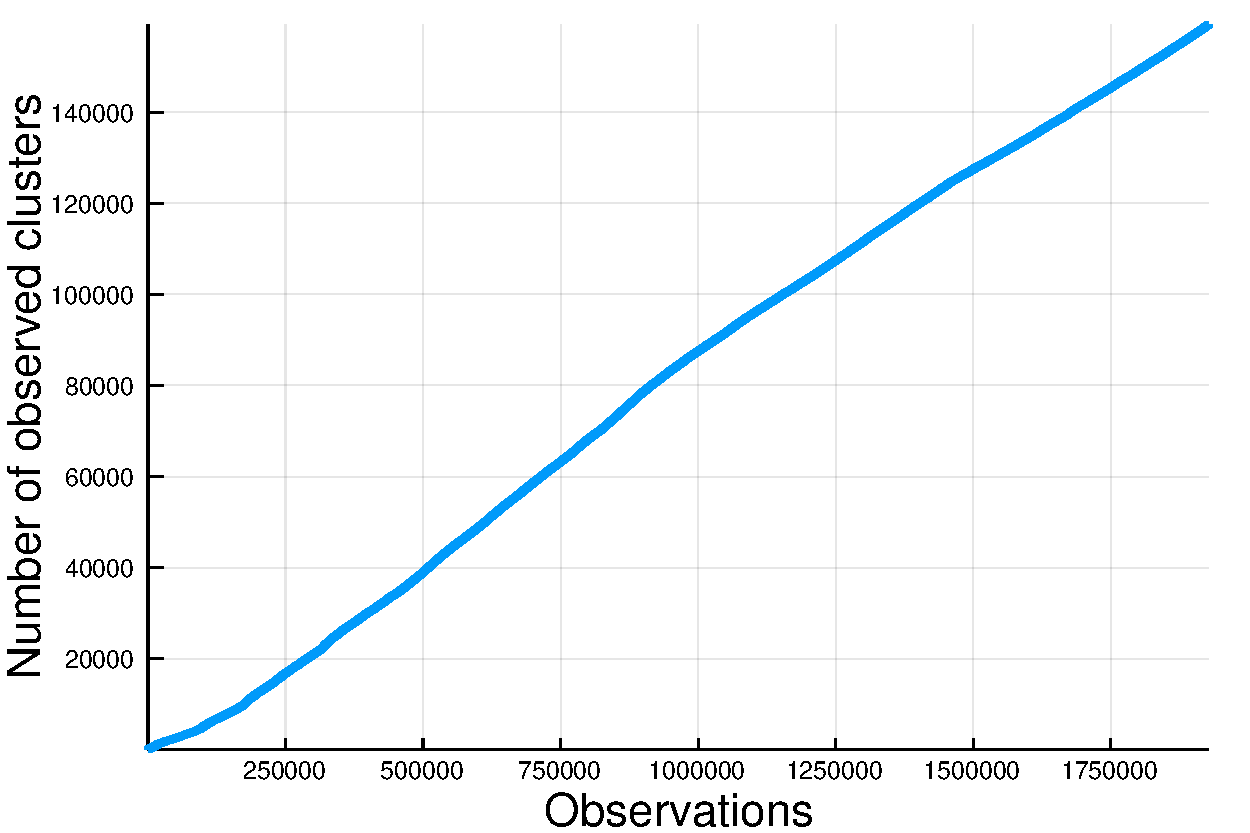
\includegraphics[width=0.8\textwidth]{fig/arrival_times_askubuntu.pdf}
	\end{figure}
	
\end{frame}

\begin{frame}
	\frametitle{Stack Overflow arrival process}
	\begin{figure}[h]
		\includegraphics[width=0.8\textwidth]{fig/arrival_times_stackoverflow.pdf}
	\end{figure}
	
\end{frame}

\begin{frame}
	\frametitle{UCI social network arrival process}
	\begin{figure}[h]
		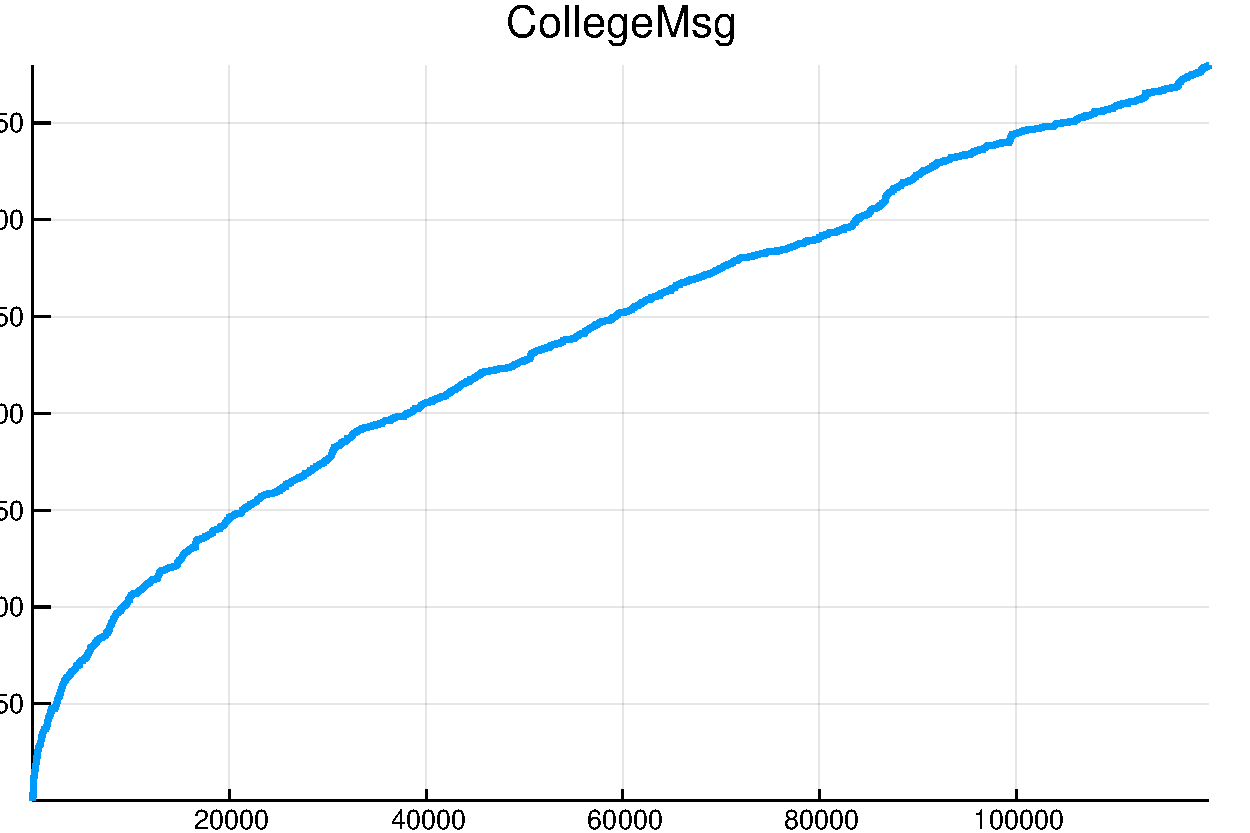
\includegraphics[width=0.8\textwidth]{fig/arrival_times_CollegeMsg.pdf}
	\end{figure}
	
\end{frame}

\begin{frame}
	\frametitle{Ask Ubuntu degree distribution}
	\begin{figure}[h]
		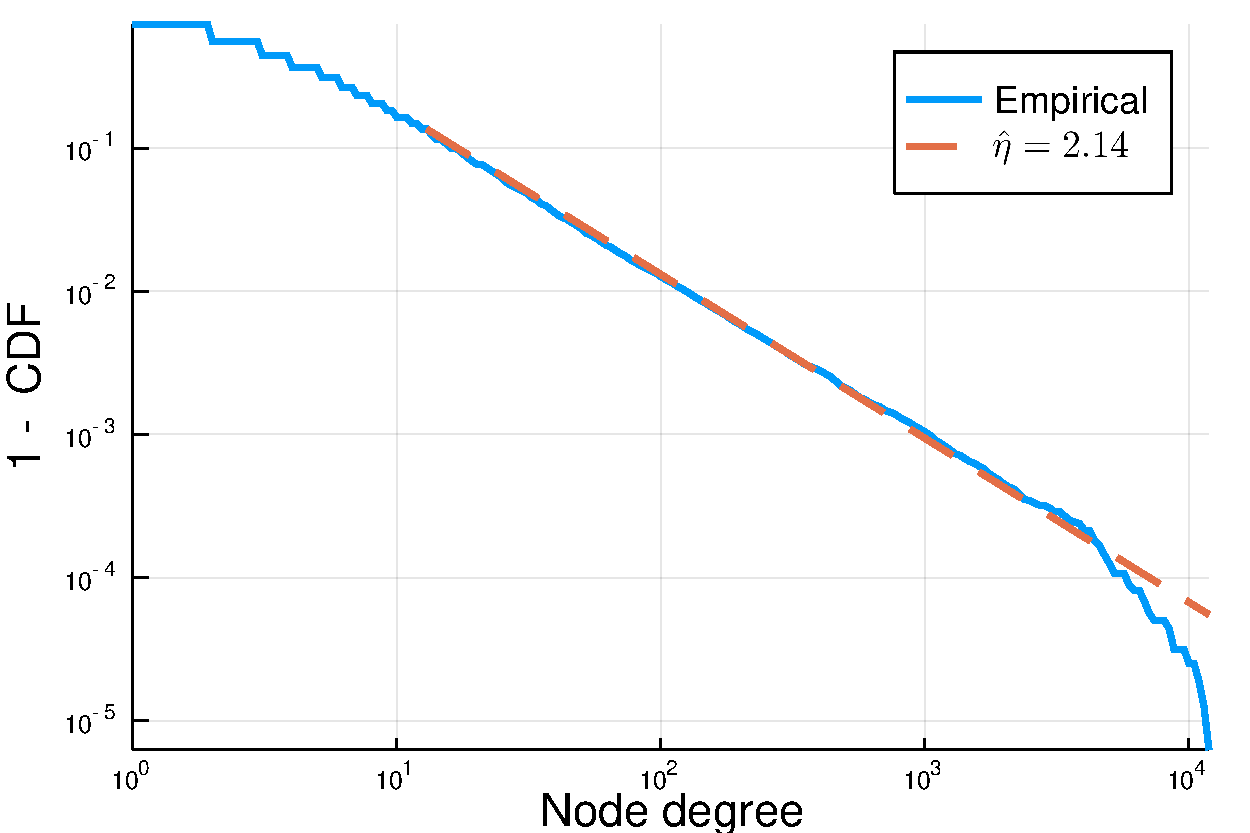
\includegraphics[width=0.8\textwidth]{fig/nodes_degre_power_law_askubuntu.pdf}
	\end{figure}
	
	Estimation used technique of \cite{clauset}
	
\end{frame}

\begin{frame}
	\frametitle{Todo}
	\begin{itemize}
		\item Recompile the images with better labels on the axes
		\item Estimate $\sigma$ by linear regression
	\end{itemize}
	
\end{frame}

\subsection{Models}
\begin{frame}
	\frametitle{Models}
	\begin{itemize}
		\item Vertex exchangeable models do not give sparsity \cite{aldous1981} \cite{hoover1979}
		\item Exchangeable point process models \cite{caronfox} have an independent notion of time
		\item \textbf{Preferential attachment models} \cite{barabasi1999}
		\item \textbf{Edge exchangeable models} \cite{CraneDempsey2017} \cite{cai2016}
	\end{itemize}
\end{frame}

\begin{frame}
	\frametitle{Yule-Simon Process}
	Parameter $\beta \in (0, 1)$.
	\vspace{15pt}
	
	Arrivals
	\begin{align}
	T_{j+1} - T_{j} \simiid \text{Geom}\left( \beta \right)
	\end{align}
	Size-biased reinforcement
	\begin{align} 
	\ee_{n+1} | \bfee_{n}, \bfT &= \begin{cases}\begin{aligned}
	K_{n+1} & \text{ w.p. } 1 && \text{if } n+1 = T_{K_{n+1}} \\
	j &\text{ w.p.} \propto d_{j,n} && \text{otherwise} 
	\end{aligned}\end{cases}
	\label{eq:ys}
	\end{align}
\end{frame}

\begin{frame}
	\frametitle{Yule-Simon Process}
	Asymptotic power law degree distribution with
	\begin{equation*}
		\eta = 1 + \frac{1}{1-\beta} > 2
	\end{equation*}
	and $K_n = O(n)$
\end{frame}

\begin{frame}
	\frametitle{Pitman-Yor Process}
	Parameters $\tau \in (0, 1), \theta > -\tau$.
	\vspace{15pt}
	
	Urn process
	\begin{align} 
	\ee_{n+1} | \bfee_{n} &= \begin{cases}\begin{aligned}
	K_{n+1} & \text{ w.p. } \frac{\theta + K_n \tau}{n + \theta}  \\
	& \\
	j &\text{ w.p. } \frac{d_{j,n} - \tau}{\theta + n} 
	\end{aligned}\end{cases}
	\label{eq:pyp1}
	\end{align}
\end{frame}

\begin{frame}
	\frametitle{Pitman-Yor Process}
	Asymptotic power law degree distribution with
	\begin{equation*}
		\eta = 1 + \tau \in (1, 2)
	\end{equation*}
	and $K_n = o(n)$
\end{frame}


\begin{frame}
	\frametitle{Edge exchangeable models \cite{cai2016}, \cite{CraneDempsey2017}}
	``The probability of all orderings of edge arrivals is the same''
	
	\vspace{20pt}
	
	$\eta \in (1,2)$
	
	$\exists$ a class of models that includes (some) edge exchangeable models, but also YS and admits all the $\eta$s
	
\end{frame}

\begin{frame}
	\frametitle{Rewriting the Pitman-Yor Process}
	Parameters $\tau \in (0, 1), \theta > -\tau$.
	\vspace{15pt}
	
	Arrivals
	\begin{align}
	\bbP(T_{j+1} - T_j > t \mid T_j) = \prod_{i=1}^{t} \frac{T_j + t - j \tau}{T_j + t + \theta}
	\end{align}
	Size-biased reinforcement
	\begin{align} 
	\ee_{n+1} | \bfee_{n}, \bfT &= \begin{cases}\begin{aligned}
	K_{n+1} & \text{ w.p. } 1 && \text{if } n+1 = T_{K_{n+1}} \\
	j &\text{ w.p.} \propto (d_{j,n} - \tau) && \text{otherwise} 
	\end{aligned}\end{cases}
	\label{eq:pyp}
	\end{align}
\end{frame}

\begin{frame}
	\frametitle{Beta Neutral-to-the-left Process \cite{Bloem2017}}
	Parameters $\alpha \in (-\infty, 1)$ and $\Lambda_\phi$ a law on $\mathbb{N}^\infty$.
	\vspace{15pt}
	
	Arrivals
	\begin{align}
	\bfT \sim \Lambda_\phi
	\end{align}
	Size-biased reinforcement
	\begin{align} 
	\ee_{n+1} | \bfee_{n}, \bfT &= \begin{cases}\begin{aligned}
	K_{n+1} & \text{ w.p. } 1 && \text{if } n+1 = T_{K_{n+1}} \\
	j &\text{ w.p.} \propto (d_{j,n} - \alpha) && \text{otherwise} 
	\end{aligned}\end{cases}
	\label{eq:bntl}
	\end{align}
\end{frame}

\begin{frame}
	\frametitle{Relationship with other model classes}
	\begin{figure}[H]
		\begin{center}
			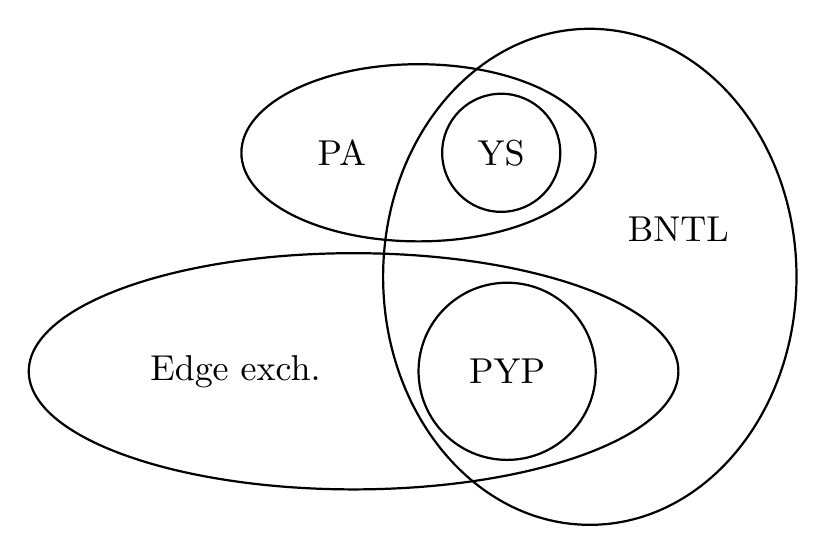
\begin{tikzpicture}[->,auto,node distance=3.6cm, thick,baseline=0,scale=0.75]
			
			\tikzstyle{every node}=[scale=1.3]
			
			\def\pyp{(-0.9,-0.2) coordinate (a) circle (1.5cm)}
			\def\ys{(-1,3.5) coordinate (b)  circle (1cm)}
			\def\ex{(-3.5,-0.2) coordinate (c) ellipse (5.5cm and 2cm)}
			\def\pa{(-2.4,3.5) coordinate (d) ellipse (3cm and 1.5cm)}
			\def\bntl{(0.5,1.4) coordinate (e) ellipse (3.5cm and 4.2cm)}
			
			\draw \pyp  node {PYP};
			\draw \ys node {YS};
			\draw \ex;
			\draw node at (-5.5,-0.2) {Edge exch.};
			\draw \pa;
			\draw node at (-3.7, 3.5) {PA};
			\draw \bntl;
			\draw node at (2,2.2) {BNTL};
			\end{tikzpicture}
		\end{center}
	\end{figure}
\end{frame}

\begin{frame}
	\frametitle{Hierarchical representation of BNTL process}
	Arrivals
	\begin{equation*}
	\bfT \sim \Lambda_\phi
	\end{equation*}
	Latent sociabilities
	\begin{equation*}
		\Psi_j | T_j \sim \text{Beta}(1-\alpha,T_j-1-(j-1)\alpha) \text{ for } j\geq 1
	\end{equation*}
	Left-neutral resampling probabilities
	\begin{align*}
		P_{j,k+1} = 
		\begin{cases}
		P_{j,k}(1-\Psi_{k+1}), & j \in \{1,\dots,k\} \\
		\Psi_{k+1}, & j = k+1
		\end{cases}
	\end{align*}
	Sampling rule
	\begin{align*} 
		\ee_{n+1} | \mathbf{P}_{K_n}, \bfT &= \begin{cases}\begin{aligned}
		K_{n+1} & \text{ w.p. } 1 && \text{if } n+1 = T_{K_{n+1}} \\
		j &\text{ w.p. } P_{j, K_n} && \text{otherwise} 
		\end{aligned}\end{cases}
	\end{align*}
\end{frame}


\section{Inference}
\subsection{Preliminaries}
\begin{frame}
	\frametitle{Observation cases}
	\begin{center}
		\begin{tabular}{ll}
			\textbf{Observation} & \textbf{Unobserved variables} \\
			\hline
			End of edge sequence $\bfee_n$ & $\alpha,\phi,\bfPsi_{K_n}$ \\
			Vertex arrival-ordered graph & $\alpha,\phi,\bfPsi_{K_n}, \bfT_{K_n}$ \\
			Unlabeled graph & $\alpha,\phi,\bfPsi_{K_n},\bfT_{K_n},\sigma [K_n]$
		\end{tabular}
	\end{center}
\end{frame}

\subsection{Gibbs sampler}
\begin{frame}
\frametitle{Sampling $\bfPsi$}

If $\bfee_n$ is observed we have a closed form for $\bfPsi$
\begin{align*}
	p_{\alpha, \phi}(\bfPsi_{K_n}| \bfee_n) = \frac{p_{\alpha, \phi}(\bfPsi_{K_n}, \bfee_n)}{p_{\alpha, \phi}(\bfee_n)},
\end{align*}
furthermore
\begin{equation*}
	\Psi_j \mid \bfee_n, \bfPsi_{\setminus j} \sim \text{Beta}(d_{j,n} - \alpha, \bar{d}_{j-1,n} - (j-1)\alpha) \;,
\end{equation*}
where
\begin{equation*}
	\bar{d}_{j,n} = \sum_{i=1}^j d_{j,n}.
\end{equation*}

\begin{itemize}
	\item For fixed $\alpha$, we have a closed form posterior
	\item Learning other variables, we have a closed form Gibbs update
\end{itemize}
\end{frame}

\begin{frame}
	\frametitle{Sampling $\alpha, \phi$}
	\begin{itemize}
		\item Place priors on $\alpha, \phi$
		\item Left with one-dimensional unnormalized density for $\alpha$ and MCMC is applicable
		\item For $\phi$, depends on $\Lambda_\phi$. Our experiments used conjugacy or slice sampling.
	\end{itemize}
	

\end{frame}

\begin{frame}
	\frametitle{Sampling $\bfT$}
	Assume
	\begin{align*}
	\boldsymbol{\aDist}^{\phi}(\bfT_k) = \delta_{T_1}(1) \prod_{j=2}^k \aDist_j^{\phi}(\Delta_j | T_{j-1}) \;,
	\end{align*}
	Support of $T_j - T_{j-1} | T_{\backslash j}$ is
	\begin{equation*}
		\{ 1, ..., \min(T_{j+1} - T_{j-1} - 1, \bar{d}_{j-1} - T_{j-1} + 1)  \}
	\end{equation*}
	Using our assumptions we can compute each conditional probability
\end{frame}

\begin{frame}
	\frametitle{Sampling $\sigma[K_n]$}
	Use Metropolis-Hastings with swap proposal $\sigma_j \leftrightarrow \sigma{j+1}$
	
	Ratio of joints from ...
\end{frame}

\begin{frame}
	\frametitle{Point estimation}
	Factorization $p_{\alpha, \phi}(\bfee_n) = p_\alpha (\bfee_n | \bfT_{K_n})\Lambda_\phi(\bfT_{K_n})$ aids MLE/MAP
\end{frame}

\begin{frame}
	\frametitle{References}
	\footnotesize{\bibliographystyle{unsrt}
	\bibliography{refs}}
\end{frame}

\end{document}
